% =====================================================================
%  SA E-Commerce Data Pipeline -- Project Documentation
%  Build:  lualatex project-documentation.tex   (run twice for TOC)
% =====================================================================
\documentclass[10pt,a4paper]{article}

% ---------- Fonts ----------
\usepackage{lmodern}
\usepackage{fontspec}
\setmainfont{Lato}[
  Ligatures=TeX,
  BoldFont={Lato Bold},
  ItalicFont={Lato Light Italic},
  BoldItalicFont={Lato Bold Italic}
]
\setsansfont{Lato}
\setmonofont{Fira Mono}[Scale=0.92, AutoFakeSlant=0.18]

% ---------- Language ----------
\usepackage[english]{babel}

% ---------- Page geometry ----------
\usepackage[
  top=25mm,
  bottom=24mm,
  left=22mm,
  right=22mm,
  headheight=19pt,
  headsep=8mm,
  footskip=12mm
]{geometry}

% ---------- Core packages ----------
\usepackage{microtype}
\usepackage{xcolor}
\usepackage{graphicx}
\usepackage{titlesec}
\usepackage{booktabs}
\usepackage{tabularx}
\usepackage{array}
\usepackage{enumitem}
\usepackage{listings}
\usepackage{tikz}
\usepackage{fancyhdr}
\usepackage[most]{tcolorbox}
\usepackage[hidelinks]{hyperref}

\usetikzlibrary{arrows.meta,positioning,calc,shapes.geometric,fit,backgrounds}

% =====================================================================
%  Design tokens
% =====================================================================
\definecolor{brand}{HTML}{0B3D2E}
\definecolor{brandmid}{HTML}{1B7F5F}
\definecolor{brandsoft}{HTML}{E8F1ED}
\definecolor{accent}{HTML}{B8862B}
\definecolor{accentsoft}{HTML}{FBF3E2}
\definecolor{ink}{HTML}{22282B}
\definecolor{muted}{HTML}{6E777D}
\definecolor{rule}{HTML}{D8DEDB}
\definecolor{codebg}{HTML}{F5F7F6}
\definecolor{codeframe}{HTML}{E2E8E5}
\definecolor{warn}{HTML}{9C3B1E}
\definecolor{warnsoft}{HTML}{FBEDE9}

% =====================================================================
%  Typography
% =====================================================================
\color{ink}
\pagestyle{fancy}
\fancyhf{}
\renewcommand{\headrulewidth}{0.4pt}
\renewcommand{\footrulewidth}{0pt}
\renewcommand{\headrule}{\hbox to\headwidth{\color{rule}\leaders\hrule height \headrulewidth\hfill}}
\fancyhead[L]{\footnotesize\color{muted}\MakeUppercase{South African E-Commerce Data Pipeline}}
\fancyhead[R]{\footnotesize\color{muted}\MakeUppercase{\leftmark}}
\fancyfoot[C]{\footnotesize\color{muted}\thepage}
\renewcommand{\sectionmark}[1]{\markboth{#1}{}}

\titleformat{\section}
  {\normalfont\Large\bfseries\color{brand}}{\thesection}{0.7em}{}
  [\vspace{2pt}\titlerule]
\titlespacing*{\section}{0pt}{18pt}{10pt}

\titleformat{\subsection}
  {\normalfont\large\bfseries\color{brandmid}}{\thesubsection}{0.6em}{}
\titlespacing*{\subsection}{0pt}{14pt}{6pt}

\titleformat{\subsubsection}
  {\normalfont\normalsize\bfseries\color{ink}}{\thesubsubsection}{0.6em}{}
\titlespacing*{\subsubsection}{0pt}{11pt}{4pt}

\setlist[itemize]{leftmargin=1.35em,itemsep=3pt,topsep=5pt,parsep=0pt}
\setlist[enumerate]{leftmargin=1.6em,itemsep=3pt,topsep=5pt,parsep=0pt}

% =====================================================================
%  Helpers
% =====================================================================
\newcommand{\cpath}[1]{\nolinkurl{#1}}
\newcommand{\chip}[1]{\textcolor{brand}{\texttt{#1}}}
\newcommand{\pill}[1]{%
  \tikz[baseline=(t.base)]\node[fill=brandsoft,text=brand,rounded corners=1.2pt,
  inner xsep=4pt,inner ysep=1.4pt,font=\footnotesize\bfseries] (t) {#1};}

% =====================================================================
%  Callout boxes
% =====================================================================
\newtcolorbox{keybox}[1][]{%
  enhanced, breakable,
  colback=brandsoft, colframe=brand,
  boxrule=0pt, leftrule=3pt,
  arc=1.4mm, left=4mm, right=3mm, top=3mm, bottom=3mm,
  fonttitle=\bfseries\small, title={#1},
  before skip=10pt, after skip=10pt}

\newtcolorbox{warnbox}[1][]{%
  enhanced, breakable,
  colback=warnsoft, colframe=warn,
  boxrule=0pt, leftrule=3pt,
  arc=1.4mm, left=4mm, right=3mm, top=3mm, bottom=3mm,
  fonttitle=\bfseries\small, title={#1},
  before skip=10pt, after skip=10pt}

\newtcolorbox{plainbox}[1][]{%
  enhanced, breakable,
  colback=white, colframe=rule,
  boxrule=0.6pt, arc=1.4mm, left=4mm, right=4mm, top=3mm, bottom=3mm,
  before skip=10pt, after skip=10pt}

% =====================================================================
%  Code listings
% =====================================================================
\lstdefinestyle{py}{
  language=Python,
  basicstyle=\ttfamily\footnotesize,
  keywordstyle=\color{brand}\bfseries,
  stringstyle=\color{accent},
  commentstyle=\color{muted}\itshape,
  emph={fetch_products,clean_products,load_products,run_report,main},
  emphstyle=\color{brandmid}\bfseries,
  numbers=none, frame=none, showstringspaces=false,
  breaklines=true, breakatwhitespace=false,
  tabsize=4, upquote=true, escapeinside={(*@}{@*)}
}
\lstdefinestyle{sh}{
  language=bash,
  basicstyle=\ttfamily\footnotesize,
  keywordstyle=\color{brand}\bfseries,
  commentstyle=\color{muted}\itshape,
  numbers=none, frame=none, showstringspaces=false,
  breaklines=true, tabsize=4, upquote=true, morekeywords={python,python3,pip,git,sqlite3,source,pytest}
}
\lstdefinestyle{txt}{
  basicstyle=\ttfamily\footnotesize,
  numbers=none, frame=none, showstringspaces=false,
  breaklines=true, tabsize=4, upquote=true,
  keywordstyle=\color{brandmid}, commentstyle=\color{muted}\itshape
}

\newtcolorbox{codebox}[1][]{%
  enhanced, breakable,
  colback=codebg, colframe=codeframe,
  boxrule=0.6pt, arc=1.2mm,
  left=3mm, right=3mm, top=2.4mm, bottom=2.4mm,
  before skip=9pt, after skip=9pt,
  before upper={\setlength{\parindent}{0pt}},
  #1}

% =====================================================================
%  Tables
% =====================================================================
\renewcommand{\arraystretch}{1.25}
\newcolumntype{Y}{>{\raggedright\arraybackslash}X}
\newcolumntype{L}[1]{>{\raggedright\arraybackslash}p{#1}}
\newcommand{\thead}[1]{\textbf{\textcolor{brand}{#1}}}

% =====================================================================
%  Hyperlinks
% =====================================================================
\hypersetup{
  colorlinks=true,
  linkcolor=brand,
  urlcolor=brandmid,
  pdftitle={SA E-Commerce Data Pipeline -- Project Documentation},
  pdfsubject={Python ETL pipeline for retail inventory analytics},
  pdfauthor={Lebo Moropene},
  pdfkeywords={data engineering, ETL, Python, pandas, SQLite, SQL, analytics, inventory}
}

% =====================================================================
%  Title page
% =====================================================================
\begin{document}

\begin{titlepage}
\thispagestyle{empty}
\begin{tikzpicture}[remember picture,overlay]
  \fill[brand] (current page.north west) rectangle ([yshift=-10.6cm]current page.north east);
  \fill[accent] ([yshift=-10.6cm]current page.north west) rectangle ([yshift=-10.25cm]current page.north east);
  \fill[brandmid,opacity=0.16]
    ([xshift=-3.2cm,yshift=-4.0cm]current page.north east)
    circle[radius=5.6cm];
  \fill[brandmid,opacity=0.10]
    ([xshift=-1.0cm,yshift=-7.4cm]current page.north east)
    circle[radius=3.4cm];
\end{tikzpicture}

\vspace*{4.6cm}

{\color{white}\fontsize{13}{16}\selectfont\bfseries\MakeUppercase{Project Documentation}\par}
\vspace{0.55cm}
{\color{white}\fontsize{33}{37}\selectfont\bfseries
South African\\[0.12cm]
E-Commerce Data Pipeline\par}
\vspace{0.7cm}
{\color{brandsoft}\fontsize{13.5}{19}\selectfont
A production-shaped Extract $\rightarrow$ Validate $\rightarrow$ Transform $\rightarrow$
Load $\rightarrow$ Analyse pipeline for retail inventory analytics.\par}

\vspace{6.0cm}

\noindent{\color{brand}\rule{\textwidth}{0.8pt}\par}
\vspace{0.5cm}

\noindent
\begin{tabularx}{\textwidth}{@{}L{3.1cm}Y@{}}
  \textcolor{muted}{Repository} &
  \cpath{git@github.com:Lebo-Moropene/sa-ecommerce-data-pipeline.git} \\[3pt]
  \textcolor{muted}{Stack} &
  Python 3.10+, \cpath{requests}, \cpath{pandas}, SQLite, SQL, \cpath{pytest} \\[3pt]
  \textcolor{muted}{Source} &
  \cpath{dummyjson.com/products} (public sample REST API) \\[3pt]
  \textcolor{muted}{Status} &
  Complete --- all four pipeline stages implemented, tested and verified end to end. \\
\end{tabularx}

\vfill

{\color{muted}\footnotesize
This document describes what the pipeline is, the problem it solves, how it is
architected, and how to install, run, extend and troubleshoot it.
It was generated from the repository source at commit
\texttt{82a4721}.}

\end{titlepage}

% =====================================================================
%  Table of contents
% =====================================================================
{\hypersetup{linkcolor=brand}%
\tableofcontents}

\newpage

% =====================================================================
% =====================================================================
%  SA E-Commerce Data Pipeline -- document body
% =====================================================================

% =====================================================================
\section{Executive Summary}
% =====================================================================

This project is a complete, working Extract--Transform--Load--Analyse (ETLA)
data engineering pipeline written in Python. It pulls a live product catalogue
from a public REST API, puts that data through a deliberate validation and
cleaning stage, loads the survivors into a SQLite database, and finally runs
three inventory and category analytics reports against the result.

The pipeline exists to answer three questions that every online retailer has
to answer continuously and correctly:

\begin{enumerate}
  \item \textbf{What is about to run out?} Which products have the lowest
        stock on hand and need replenishment first.
  \item \textbf{What does the catalogue look like?} How the assortment is
        distributed across categories, which tells you about shelf space,
        merchandising effort and marketing focus.
  \item \textbf{How is the catalogue priced?} The average price point per
        category, which tells you about price positioning and leaves room for
        promotional strategy.
\end{enumerate}

What separates this from a script that calls an API and prints a table is the
middle of the pipeline. Data arriving from an API is untrusted: fields are
missing, numbers arrive as strings, titles are blank, and identifiers repeat.
The pipeline treats that as the normal case rather than the exception. Every
record is checked against an explicit rule set, and anything that fails is
routed to a \emph{reject file} with the reason implied by the rule it broke.
Nothing is silently dropped, and nothing unvalidated ever reaches the
database.

The project is deliberately small and dependency-light --- four runtime
packages, one file per pipeline stage, and a SQLite file you can open with
the \cpath{sqlite3} command-line tool on any machine --- which makes it easy
to read end to end, easy to demonstrate, and easy to extend with more
sources or more reports.

\subsection{At a glance}

\noindent
\begin{tabularx}{\textwidth}{@{}L{4.1cm}Y@{}}
\thead{Language}         & Python 3.10 or newer \\
\thead{Pipeline stages}  & Extract $\rightarrow$ Validate/Transform $\rightarrow$ Load $\rightarrow$ Analyse \\
\thead{Runtime deps}     & \cpath{requests}, \cpath{pandas} \\
\thead{Test dependency}  & \cpath{pytest} \\
\thead{Data store}       & SQLite (single file, \cpath{data/ecommerce.db}) \\
\thead{Analytics}        & 3 reports, written in SQL and executed in the database layer \\
\thead{Tests}            & 3 automated tests covering the three report queries \\
\thead{Entry point}      & \cpath{python -m src.pipeline} \\
\thead{Lines of Python}  & 5 modules, 4 pipeline stages plus the orchestrator \\
\thead{Repository}       & \cpath{git@github.com:Lebo-Moropene/sa-ecommerce-data-pipeline.git} \\
\end{tabularx}

% =====================================================================
\section{The Problem This Pipeline Solves}
% =====================================================================

\subsection{The business problem}

South African e-commerce operators face the same inventory pressure as any
competitive online retailer, and the pressure shows up in three concrete
places.

\textbf{Stockouts.} A product that is out of stock does not generate a slow
sale --- it generates no sale at all, and it quietly pushes the customer to a
competitor. The catalogue in this pipeline contains a wireless charger with
a single unit left. Nothing about that record looks urgent in a raw JSON feed.
It only becomes urgent once it is ranked, aggregated and presented next to
everything else that is low.

\textbf{Blind spots in the assortment.} A buyer or merchandiser needs to know
whether the catalogue is well balanced or lopsided. If five hundred of the
products are in one category, the category is the store and the other
categories are shelf dressing. A simple count per category surfaces that
immediately --- but only if the data is clean enough to count.

\textbf{Price positioning.} Average price per category is the cheapest way
to see whether the assortment sits in the premium or the budget tier, and
therefore where promotions, bundles or supplier negotiations will pay off.

\subsection{The technical problem}

The business questions are easy to state and awkward to answer with dirty
data. A live product API returns records with missing brands, prices encoded
as strings, blank titles, duplicated identifiers and negative stock levels.
Any analysis written directly against that payload produces confident,
well-formatted, quietly wrong answers --- because the aggregation ran over
rows that should never have been counted.

This is the failure mode the pipeline is engineered to prevent. The
validation stage sits between extraction and analysis specifically so that
the reports operate on a dataset whose contents are known and auditable.

\subsection{Problem to solution}

\noindent
\begin{tabularx}{\textwidth}{@{}L{3.6cm}L{3.9cm}Y@{}}
\thead{Problem} & \thead{Why it hurts} & \thead{How this pipeline handles it} \\
\midrule
Stock running low is invisible in a raw feed &
Replenishment happens after the stockout, not before it &
Ranks products by stock ascending and prints the five closest to running out \\
\addlinespace
Catalogue is skewed by category &
Merchandising and marketing effort is misallocated &
Counts products per category and orders by volume \\
\addlinespace
Price positioning is unknown &
Promotions are priced by gut feel &
Averages price per category and orders by price point \\
\addlinespace
API records are incomplete or invalid &
Reports quietly aggregate nonsense &
Nine validation rules reject bad rows to an auditable CSV \\
\addlinespace
Re-running the pipeline duplicates rows &
Counts inflate on every run &
The load step replaces the table rather than appending to it \\
\addlinespace
The pipeline only works from one directory &
Breaks the moment it is scheduled from elsewhere &
Every path is resolved relative to the source file, not the shell's CWD \\
\end{tabularx}

\begin{keybox}[The core design decision]
Data quality is enforced \emph{before} analysis, not alongside it. A rejected
record never reaches the database, so it can never be counted, averaged or
ranked. Every rejection is written to
\cpath{data/rejected/rejected_products.csv} so that the volume and nature of
bad data is itself a reportable signal.
\end{keybox}

% =====================================================================
\section{How It Works}
% =====================================================================

\subsection{Architecture at a glance}

The pipeline is a linear sequence of four stages. Each stage is a standalone
module with a single public function, reads from one location and writes to
another, and can be executed on its own --- which is what makes the pipeline
debuggable: you can re-run just the stage that broke and keep the results of
the ones before it.

\begin{center}
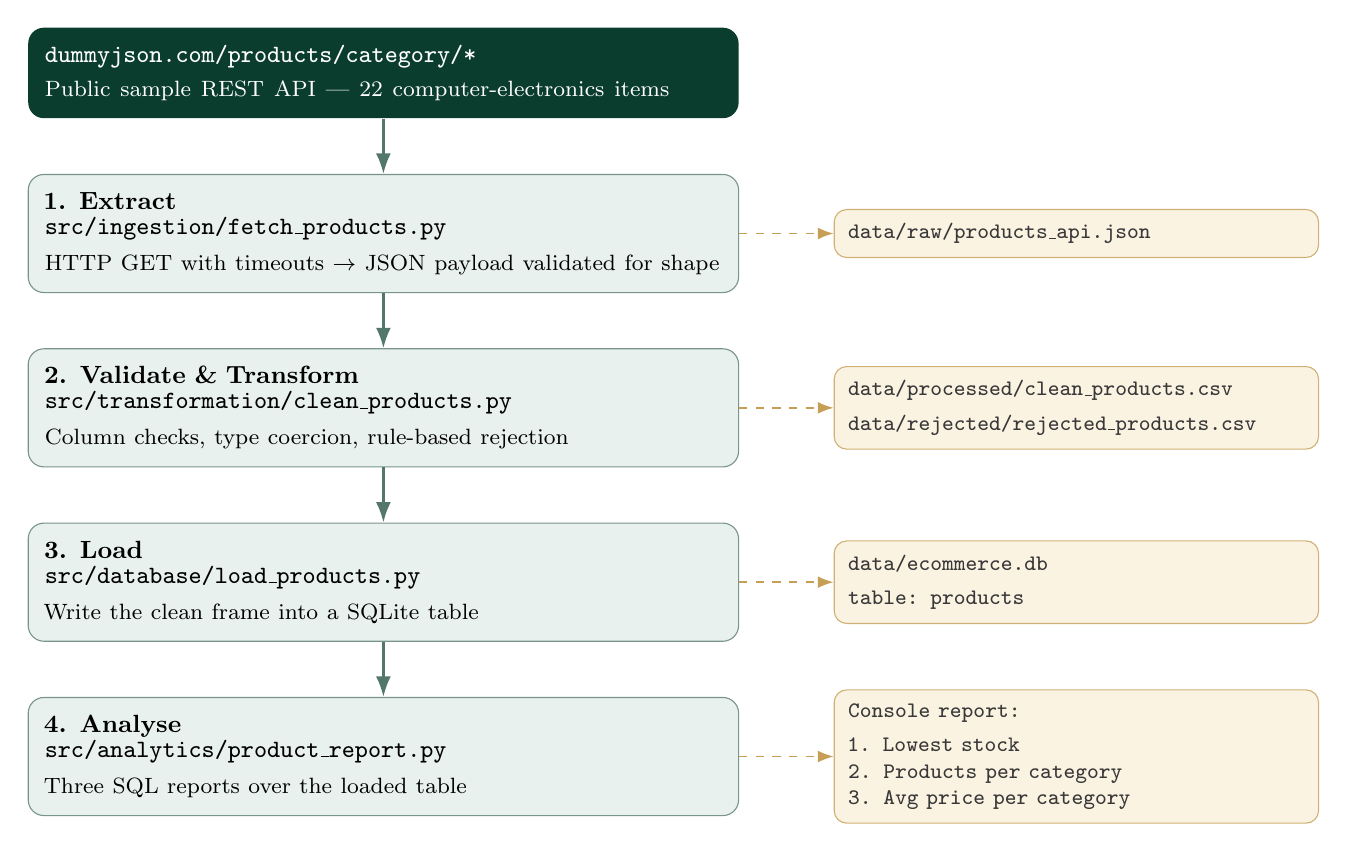
\begin{tikzpicture}[
  node distance=7mm,
  src/.style={rectangle, rounded corners=2mm, fill=brand, text=white,
    text width=8.6cm, minimum height=1.15cm, align=left, inner sep=6pt,
    font=\small\bfseries},
  stage/.style={rectangle, rounded corners=2mm, draw=brand!55, fill=brandsoft,
    text width=8.6cm, minimum height=1.5cm, align=left, inner sep=6pt,
    font=\small},
  artifact/.style={rectangle, rounded corners=1.6mm, draw=accent!65, fill=accentsoft,
    text width=5.8cm, align=left, inner sep=5pt, font=\footnotesize\ttfamily,
    text=black!78},
  flow/.style={-{Latex[length=2.6mm,width=1.9mm]}, brand!70, line width=0.9pt},
  side/.style={-{Latex[length=2mm,width=1.5mm]}, accent!80, line width=0.6pt, dashed}
]
\node[src] (source) {\texttt{dummyjson.com/products/category/*}\\[1pt]
  {\footnotesize\normalfont Public sample REST API --- 22 computer-electronics items}};

\node[stage, below=of source] (s1) {
  \textbf{1. Extract}\\[-2pt]
  \texttt{src/ingestion/fetch\_products.py}\\[2pt]
  {\footnotesize\normalfont HTTP GET with timeouts $\rightarrow$ JSON payload validated for shape}};

\node[artifact, right=12mm of s1] (a1) {data/raw/products\_api.json};

\node[stage, below=of s1] (s2) {
  \textbf{2. Validate \& Transform}\\[-2pt]
  \texttt{src/transformation/clean\_products.py}\\[2pt]
  {\footnotesize\normalfont Column checks, type coercion, rule-based rejection}};

\node[artifact, right=12mm of s2] (a2) {data/processed/clean\_products.csv\\[3pt]
  data/rejected/rejected\_products.csv};

\node[stage, below=of s2] (s3) {
  \textbf{3. Load}\\[-2pt]
  \texttt{src/database/load\_products.py}\\[2pt]
  {\footnotesize\normalfont Write the clean frame into a SQLite table}};

\node[artifact, right=12mm of s3] (a3) {data/ecommerce.db\\[3pt] table: products};

\node[stage, below=of s3] (s4) {
  \textbf{4. Analyse}\\[-2pt]
  \texttt{src/analytics/product\_report.py}\\[2pt]
  {\footnotesize\normalfont Three SQL reports over the loaded table}};

\node[artifact, right=12mm of s4] (a4) {Console report:\\[3pt]
  1. Lowest stock\\ 2. Products per category\\ 3. Avg price per category};

\draw[flow] (source) -- (s1);
\draw[flow] (s1) -- (s2);
\draw[flow] (s2) -- (s3);
\draw[flow] (s3) -- (s4);

\draw[side] (s1.east) -- (a1.west);
\draw[side] (s2.east) -- (a2.west);
\draw[side] (s3.east) -- (a3.west);
\draw[side] (s4.east) -- (a4.west);
\end{tikzpicture}
\end{center}

\subsection{Stage 1 --- Extract}

\cpath{src/ingestion/fetch_products.py} issues one HTTP GET per category
against the catalogue endpoint, then merges the responses into a single
payload.

\begin{codebox}
\noindent
\begin{lstlisting}[style=py]
API_BASE_URL = "https://dummyjson.com/products/category"
API_CATEGORIES = ["laptops", "tablets", "mobile-accessories"]

for category in API_CATEGORIES:
    url = f"{API_BASE_URL}/{category}"

    response = requests.get(url, timeout=(5, 15))
    response.raise_for_status()
    payload = response.json()

    category_products = payload.get("products")
    if not isinstance(category_products, list):
        raise SystemExit("Unexpected API response: products list is missing.")

    products.extend(category_products)
    total += payload.get("total", len(category_products))
\end{lstlisting}
\end{codebox}

The three responses are merged, untouched, into a single payload and written
to \cpath{data/raw/products_api.json} before any interpretation happens.
Keeping the untransformed payload on disk means the extraction stage is
reproducible: if a later stage produces a surprising result, the exact rows
that produced it are still there.

The function is defensive about everything it does not control. Network
failures, HTTP error statuses and malformed JSON are all caught and
re-raised as a \cpath{SystemExit} with a readable message rather than a
traceback; and the decoded JSON is checked to be an object containing a
list of products before it is trusted.

\begin{warnbox}[Failure modes]
\begin{itemize}
  \item \cpath{requests.RequestException} $\rightarrow$ \emph{HTTP request failed: \ldots}
  \item Non-JSON body $\rightarrow$ \emph{API returned invalid JSON: \ldots}
  \item Payload that is not an object, or has no \cpath{products} list
        $\rightarrow$ \emph{Unexpected API response: \ldots}
\end{itemize}
\end{warnbox}

\subsection{Stage 2 --- Validate and Transform}

\cpath{src/transformation/clean_products.py} loads the raw payload into a
\cpath{pandas} DataFrame and applies the rule set described in
Section~\ref{sec:validation}. Records that satisfy every rule become the
clean dataset; the rest are written to the reject file.

\begin{codebox}
\noindent
\begin{lstlisting}[style=py]
required_columns = ["id", "title", "category", "price", "stock"]
for column in required_columns:
    if column not in df.columns:
        raise ValueError(f"Required column is missing: {column}")

df["price"] = pd.to_numeric(df["price"], errors="coerce")
df["stock"] = pd.to_numeric(df["stock"], errors="coerce")

invalid_rows = (
    df["id"].isna()
    | df["title"].isna()
    | df["title"].astype(str).str.strip().eq("")
    | df["category"].isna()
    | df["price"].isna()
    | df["stock"].isna()
    | (df["price"] < 0)
    | (df["stock"] < 0)
    | df["id"].duplicated(keep="first")
)

rejected = df[invalid_rows].copy()
clean = df[~invalid_rows].copy()
\end{lstlisting}
\end{codebox}

Two details are worth calling out. First, \cpath{errors="coerce"} is what
makes the numeric checks reliable: a price of \cpath{"not a number"} becomes
\cpath{NaN} rather than raising, and the existing \cpath{isna()} test then
rejects it. The pipeline coerces first and judges second, so no malformed
value can leak past a comparison. Second, the duplicate check uses
\cpath{duplicated(keep="first")}, which retains the first occurrence and
rejects only the repeats --- the opposite of the naive
\cpath{keep="last"} behaviour, which would silently prefer the newer record.

\subsection{Stage 3 --- Load}

\cpath{src/database/load_products.py} writes the clean frame into a SQLite
database using \cpath{pandas}' \cpath{to_sql} helper.

\begin{codebox}
\noindent
\begin{lstlisting}[style=py]
df = pd.read_csv(CSV_PATH)

with sqlite3.connect(DATABASE_PATH) as connection:
    df.to_sql("products", connection, if_exists="replace", index=False)

    count = connection.execute(
        "SELECT COUNT(*) FROM products"
    ).fetchone()[0]
\end{lstlisting}
\end{codebox}

\cpath{if_exists="replace"} is what makes the pipeline idempotent. Every run
rebuilds the \cpath{products} table from the current clean file, so running
the pipeline ten times gives the same twenty-two rows --- not two hundred and
twenty-two. The stage
also refuses to invent data: if the clean CSV does not exist it raises
\cpath{FileNotFoundError} with a message telling you to run the cleaning
step first, rather than quietly loading an empty table.

\subsection{Stage 4 --- Analyse}

\cpath{src/analytics/product_report.py} runs three queries against the
loaded database and prints the results. The analysis lives in SQL, executed
by SQLite, rather than in Python --- the database does the aggregation, and
the Python layer only formats the output. Section~\ref{sec:analytics}
covers each report in detail.

\subsection{Orchestration}

\cpath{src/pipeline.py} chains the four stages together. It is deliberately
thin: four calls in order, a banner before each step, and a completion
message at the end.

\begin{codebox}
\noindent
\begin{lstlisting}[style=py]
def main():
    print("\nSTEP 1: Fetching product data")
    fetch_products()

    print("\nSTEP 2: Cleaning product data")
    clean_products()

    print("\nSTEP 3: Loading products into SQLite")
    load_products()

    print("\nSTEP 4: Running analytics")
    run_report()

    print("\nPipeline completed successfully.")
\end{lstlisting}
\end{codebox}

Because every stage is an ordinary importable function with no shared state,
the orchestrator is a convenience, not a dependency. Running
\cpath{python -m src.ingestion.fetch_products} by hand produces exactly the
same artefact as running the full pipeline.

% =====================================================================
\section{Technology Stack}
% =====================================================================

\noindent
\begin{tabularx}{\textwidth}{@{}L{3.3cm}L{4.3cm}Y@{}}
\thead{Layer} & \thead{Tool} & \thead{Why it was chosen} \\
\midrule
Language & Python 3.10+ & The dominant language for data work; readable for
  anyone who has not written Python before, and the language the source API
  ecosystem is built on. \\
\addlinespace
Ingestion & \cpath{requests} & A mature HTTP client with first-class timeout
  support and clear exception types, which is what makes the error handling
  in Stage 1 straightforward. \\
\addlinespace
Transformation & \cpath{pandas} & Vectorised column operations turn nine
  validation rules into a single boolean mask, and the DataFrame is a
  natural fit for reading and writing CSV. \\
\addlinespace
Storage & SQLite & A single file, zero server setup, and a full SQL engine.
  The database is easy to inspect with the \cpath{sqlite3} CLI, which makes
  the analysis stage transparent rather than a black box. \\
\addlinespace
Analytics & SQL & Aggregation stays in the database where it belongs, and
  the three reports are short enough to read in full. \\
\addlinespace
Testing & \cpath{pytest} & Minimal fixtures, plain asserts, and a test
  suite that runs in under a tenth of a second. \\
\addlinespace
Version control & Git / GitHub & Branch-per-feature history, and a remote
  that anyone can clone and run. \\
\end{tabularx}

The whole runtime footprint is \cpath{requests}, \cpath{pandas} and the
Python standard library. There is no ORM, no framework, no scheduler, no
configuration file and no secrets to manage. For a pipeline this size that
is a feature: there is nothing to learn before you can run it.

% =====================================================================
\section{Repository Layout}
% =====================================================================

\begin{codebox}
\noindent
\begin{lstlisting}[style=txt]
.
|-- .gitignore                # excludes venv, caches and generated data
|-- README.md                 # quick-start guide
|-- requirements.txt          # requests, pandas, pytest
|
|-- data/
|   |-- raw/                  # API responses          (gitignored)
|   |-- processed/            # cleaned CSV output      (gitignored)
|   |-- rejected/             # rows that failed checks (gitignored)
|   `-- ecommerce.db          # SQLite database         (gitignored)
|
|-- docs/                     # project documentation
|-- logs/                     # pipeline logs           (gitignored)
|-- sql/                      # ad-hoc SQL queries
|
|-- src/
|   |-- __init__.py
|   |-- pipeline.py           # end-to-end orchestrator
|   |-- ingestion/
|   |   |-- __init__.py
|   |   `-- fetch_products.py     # Stage 1
|   |-- transformation/
|   |   |-- __init__.py
|   |   `-- clean_products.py     # Stage 2
|   |-- database/
|   |   |-- __init__.py
|   |   `-- load_products.py      # Stage 3
|   `-- analytics/
|       |-- __init__.py
|       `-- product_report.py     # Stage 4
|
`-- tests/
    `-- test_product_report.py    # pytest suite
\end{lstlisting}
\end{codebox}

\subsection{How the layout is organised}

The \cpath{src} tree mirrors the pipeline itself: one package per stage, one
module per stage, named for what it does rather than for a technical layer.
Each package has an \cpath{__init__.py} so that it is importable, and
each module exposes exactly one public function with the same name as its
purpose --- \cpath{fetch_products}, \cpath{clean_products},
\cpath{load_products}, \cpath{run_report}.

The \cpath{data} tree separates artefacts by their position in the pipeline
rather than by file type: everything the API produced lives in \cpath{raw},
everything that passed validation lives in \cpath{processed}, and everything
that failed lives in \cpath{rejected}. When you open a directory you know
immediately which stage produced the file and what its status is.

\subsection{What is not in version control}

\cpath{.gitignore} excludes the virtual environment, Python bytecode caches,
the pytest cache, IDE settings and --- importantly --- all generated data
files. Only the code, the documentation and empty-directory placeholders are
committed. This keeps the repository small and reviewable, and it means a
fresh clone is a clean slate: the \cpath{data} directories exist, ready to
be filled by the first pipeline run.

% =====================================================================
\section{Getting Started}
% =====================================================================

\subsection{Prerequisites}

\noindent
\begin{tabularx}{\textwidth}{@{}L{4.4cm}Y@{}}
\thead{Requirement} & \thead{Details} \\
\midrule
Python 3.10 or newer & Check with \cpath{python3 --version}. \\
Git & Needed only to clone the repository. \\
Network access & The pipeline calls a live public API. \\
\cpath{sqlite3} CLI & Optional --- only for ad-hoc queries in Section~\ref{sec:manual-queries}. \\
\end{tabularx}

\subsection{Clone and set up}

\begin{codebox}
\noindent
\begin{lstlisting}[style=sh]
git clone git@github.com:Lebo-Moropene/sa-ecommerce-data-pipeline.git
cd sa-ecommerce-data-pipeline

python3 -m venv .venv
source .venv/bin/activate
pip install -r requirements.txt
\end{lstlisting}
\end{codebox}

The virtual environment keeps the three dependencies isolated from the
system Python, and it is the reason \cpath{.venv/} is the first entry in
\cpath{.gitignore}. On Windows, activate with
\cpath{.venv\textbackslash Scripts\textbackslash activate} instead.

\subsection{Verify the installation}

Before running the pipeline, confirm the dependencies resolved correctly:

\begin{codebox}
\noindent
\begin{lstlisting}[style=sh]
python -m pytest tests/ -v
\end{lstlisting}
\end{codebox}

\begin{codebox}
\noindent
\begin{lstlisting}[style=txt]
platform linux -- Python 3.10.12, pytest-9.1.1
collected 3 items

tests/test_product_report.py::test_products_are_counted_by_category PASSED [ 33%]
tests/test_product_report.py::test_lowest_stock_product_is_returned_first PASSED [ 66%]
tests/test_product_report.py::test_average_price_is_calculated_correctly PASSED [100%]

============================== 3 passed in 0.02s ==============================
\end{lstlisting}
\end{codebox}

A green suite here means the environment is sound and the report queries
behave as expected --- before you add network variables into the picture.

% =====================================================================
\section{Usage Guide}
% =====================================================================

\subsection{Run the whole pipeline}

\begin{codebox}
\noindent
\begin{lstlisting}[style=sh]
python -m src.pipeline
\end{lstlisting}
\end{codebox}

This is the single command that matters. It runs all four stages in order
and prints the real output of the run --- the console report in
Section~\ref{sec:analytics} is the literal output of the command below,
captured from a live run against the public API.

\begin{codebox}
\noindent
\begin{lstlisting}[style=txt]
STEP 1: Fetching product data
HTTP status: 200 (laptops)
Products retrieved from laptops: 5
HTTP status: 200 (tablets)
Products retrieved from tablets: 3
HTTP status: 200 (mobile-accessories)
Products retrieved from mobile-accessories: 14
Products retrieved: 22
Total products reported by API: 22
Raw data saved to: .../data/raw/products_api.json

STEP 2: Cleaning product data
Products received: 22
Clean products: 22
Rejected products: 0
Clean data saved to: .../data/processed/clean_products.csv
Rejected data saved to: .../data/rejected/rejected_products.csv

STEP 3: Loading products into SQLite
Products loaded into database: 22
Database saved to: .../data/ecommerce.db

STEP 4: Running analytics

=== 1. PRODUCTS WITH LOWEST STOCK ===
Apple Airpower Wireless Charger | mobile-accessories | Stock: 1
Apple MagSafe Battery Pack | mobile-accessories | Stock: 1
Selfie Stick Monopod | mobile-accessories | Stock: 11
TV Studio Camera Pedestal | mobile-accessories | Stock: 15
Apple MacBook Pro 14 Inch Space Grey | laptops | Stock: 24

=== 2. PRODUCTS PER CATEGORY ===
mobile-accessories: 14 products
laptops: 5 products
tablets: 3 products

=== 3. AVERAGE PRICE PER CATEGORY ===
laptops: 1559.99
tablets: 483.32
mobile-accessories: 146.99

Pipeline completed successfully.
\end{lstlisting}
\end{codebox}

Two numbers in that output are worth pausing on.
\cpath{Products retrieved: 22} is how many rows came back across the three
category requests. \cpath{Total products reported by API: 22} is the size
of the computer-electronics slice the API knows about --- the catalogue as a
whole holds 194 products, but only these three categories are in scope. The
pipeline deliberately fetches one narrow slice: the point of the project is
the architecture, not the volume of data, and a twenty-two-row payload keeps
every stage and every report readable.

\subsection{Run a single stage}

Each stage is a standalone module. This is the primary debugging technique:
if the report looks wrong, re-run just the stage that produced its input
and inspect the intermediate file.

\begin{codebox}
\noindent
\begin{lstlisting}[style=sh]
python -m src.ingestion.fetch_products    # Stage 1 -> data/raw/
python -m src.transformation.clean_products   # Stage 2 -> data/processed/, data/rejected/
python -m src.database.load_products     # Stage 3 -> data/ecommerce.db
python -m src.analytics.product_report  # Stage 4 -> console report
\end{lstlisting}
\end{codebox}

\subsection{Inspect the intermediate artefacts}

\begin{codebox}
\noindent
\begin{lstlisting}[style=sh]
# the 22 rows that survived validation
cat data/processed/clean_products.csv

# anything that failed a rule (empty when the source is clean)
cat data/rejected/rejected_products.csv

# the loaded table
sqlite3 data/ecommerce.db ".tables"
sqlite3 data/ecommerce.db "SELECT COUNT(*) FROM products;"
\end{lstlisting}
\end{codebox}

\begin{codebox}
\noindent
\begin{lstlisting}[style=txt]
id,title,category,brand,price,stock,rating
78,Apple MacBook Pro 14 Inch Space Grey,laptops,Apple,1999.99,24,3.65
79,Asus Zenbook Pro Dual Screen Laptop,laptops,Asus,1799.99,45,3.95
80,Huawei Matebook X Pro,laptops,Huawei,1399.99,75,4.98
81,Lenovo Yoga 920,laptops,Lenovo,1099.99,40,2.86
82,New DELL XPS 13 9300 Laptop,laptops,Dell,1499.99,74,2.67
159,iPad Mini 2021 Starlight,tablets,Apple,499.99,47,3.18
160,Samsung Galaxy Tab S8 Plus Grey,tablets,Samsung,599.99,62,4.68
161,Samsung Galaxy Tab White,tablets,Samsung,349.99,92,3.72
99,Amazon Echo Plus,mobile-accessories,Amazon,99.99,61,4.99
100,Apple Airpods,mobile-accessories,Apple,129.99,67,4.15
101,Apple AirPods Max Silver,mobile-accessories,Apple,549.99,59,3.47
102,Apple Airpower Wireless Charger,mobile-accessories,Apple,79.99,1,3.68
103,Apple HomePod Mini Cosmic Grey,mobile-accessories,Apple,99.99,27,4.62
104,Apple iPhone Charger,mobile-accessories,Apple,19.99,31,4.15
105,Apple MagSafe Battery Pack,mobile-accessories,Apple,99.99,1,3.62
106,Apple Watch Series 4 Gold,mobile-accessories,Apple,349.99,33,2.74
107,Beats Flex Wireless Earphones,mobile-accessories,Beats,49.99,50,4.24
108,iPhone 12 Silicone Case with MagSafe Plum,mobile-accessories,Apple,29.99,69,3.62
109,Monopod,mobile-accessories,TechGear,19.99,48,4.43
110,Selfie Lamp with iPhone,mobile-accessories,GadgetMaster,14.99,58,3.55
111,Selfie Stick Monopod,mobile-accessories,SnapTech,12.99,11,3.88
112,TV Studio Camera Pedestal,mobile-accessories,ProVision,499.99,15,2.78
\end{lstlisting}
\end{codebox}

\subsection{Run the tests}

\begin{codebox}
\noindent
\begin{lstlisting}[style=sh]
python -m pytest tests/ -v      # verbose
python -m pytest tests/ -q      # quiet
python -m pytest tests/ --tb=short   # shorter tracebacks on failure
\end{lstlisting}
\end{codebox}

\subsection{Query the database yourself}
\label{sec:manual-queries}

Because the data lands in a real SQLite file, you are not limited to the
three built-in reports. Open the database and ask it anything.

\begin{codebox}
\noindent
\begin{lstlisting}[style=sh]
sqlite3 data/ecommerce.db "SELECT category, AVG(price) FROM products GROUP BY category;"

sqlite3 data/ecommerce.db "SELECT title, stock FROM products WHERE stock < 50 ORDER BY stock;"

sqlite3 data/ecommerce.db "SELECT brand, COUNT(*) FROM products GROUP BY brand ORDER BY 2 DESC;"

sqlite3 data/ecommerce.db ".schema products"
\end{lstlisting}
\end{codebox}

\begin{codebox}
\noindent
\begin{lstlisting}[style=txt]
laptops|1559.99
mobile-accessories|146.99
tablets|483.323333333333
\end{lstlisting}
\end{codebox}

% =====================================================================
\section{Data Model and Artefacts}
% =====================================================================

\subsection{Files produced by a run}

\noindent
\begin{tabularx}{\textwidth}{@{}L{5.5cm}L{2.6cm}Y@{}}
\thead{Artefact} & \thead{Produced by} & \thead{Contents} \\
\midrule
\cpath{data/raw/products_api.json} & Stage 1 &
The merged API payload, including metadata such as the catalogue total. \\
\addlinespace
\cpath{data/processed/clean_products.csv} & Stage 2 &
Every record that passed all validation rules, in the canonical column order. \\
\addlinespace
\cpath{data/rejected/rejected_products.csv} & Stage 2 &
Every record that failed a rule, with the full original row so the failure
can be diagnosed. \\
\addlinespace
\cpath{data/ecommerce.db} & Stage 3 &
A SQLite database containing the \cpath{products} table. \\
\end{tabularx}

The clean CSV keeps exactly seven columns, in a fixed order:
\cpath{id}, \cpath{title}, \cpath{category}, \cpath{brand}, \cpath{price},
\cpath{stock}, \cpath{rating}. Everything else the API sends ---
descriptions, discount percentages, SKU, weight, dimensions, warranty
information, shipping information, availability status, reviews, return
policy, minimum order quantity, metadata and image URLs --- is discarded.
That is intentional: the pipeline stores what the analytics need and the
business asks about, rather than a copy of everything the API happens to
return.

\subsection{The products table}

The schema is inferred by \cpath{pandas} from the clean CSV, so it follows
the data rather than being declared separately. The table is called
\cpath{products}:

\begin{codebox}
\noindent
\begin{lstlisting}[style=txt]
CREATE TABLE "products" (
"id"       INTEGER,
"title"    TEXT,
"category" TEXT,
"brand"    TEXT,
"price"    REAL,
"stock"    INTEGER,
"rating"   REAL
)
\end{lstlisting}
\end{codebox}

\noindent
\begin{tabularx}{\textwidth}{@{}L{2.4cm}L{2.0cm}Y@{}}
\thead{Column} & \thead{Type} & \thead{Meaning and rules} \\
\midrule
\cpath{id} & INTEGER & Product identifier from the API. Unique --- the first occurrence wins, later duplicates are rejected. \\
\cpath{title} & TEXT & Display name. Never null and never blank after stripping whitespace. \\
\cpath{category} & TEXT & Catalogue grouping, used by reports 2 and 3. \\
\cpath{brand} & TEXT & Manufacturer. Missing values are filled with the literal \cpath{Unknown} rather than being rejected. \\
\cpath{price} & REAL & Unit price. Numeric, non-negative. Used by report 3. \\
\cpath{stock} & INTEGER & Units on hand. Numeric, non-negative. Used by report 1. \\
\cpath{rating} & REAL & Customer rating. Optional --- a missing rating does not cause a rejection. \\
\end{tabularx}

\subsection{Data types and coercion}
\label{sec:coercion}

\cpath{price} and \cpath{stock} arrive from the API as whatever the producer
chose to send. The pipeline coerces both with \cpath{pd.to_numeric(...,
errors="coerce")} before any validation, which produces exactly the
behaviour you want: a well-formed number stays a number, and anything
unparseable becomes \cpath{NaN} and is then rejected by the standard
missing-value rule. There is no third path where a malformed value survives
as a string.

% =====================================================================
\section{Data Quality: Validation Rules}
\label{sec:validation}

\subsection{The rule set}

A record is written to the reject file if it breaks any of the following.

\noindent
\begin{tabularx}{\textwidth}{@{}L{1.2cm}L{5.6cm}Y@{}}
\thead{\#} & \thead{Rule} & \thead{Why it matters} \\
\midrule
1 & \cpath{id} is missing & The identifier is the key; a record without it cannot be deduplicated or referenced. \\
2 & \cpath{title} is missing & A product with no name cannot be presented to a buyer or a buyer-facing report. \\
3 & \cpath{title} is blank or whitespace-only & Semantically identical to a missing title, but survives an \cpath{isna()} check, so it needs its own rule. \\
4 & \cpath{category} is missing & Category drives two of the three reports. \\
5 & \cpath{price} is missing or not numeric & Unparseable prices become \cpath{NaN} during coercion and are caught here. \\
6 & \cpath{stock} is missing or not numeric & The same, for the field that drives the replenishment report. \\
7 & \cpath{price} is negative & A negative price is a sign error or a malformed discount, not a real price. \\
8 & \cpath{stock} is negative & Negative stock is always a data defect and would corrupt the low-stock ranking. \\
9 & \cpath{id} is a duplicate & Duplicate rows would double-count every aggregate that touches them. \\
\end{tabularx}

Rules 5 and 6 in the table cover the numeric-coercion failures described in
Section~\ref{sec:coercion}: a value that cannot be parsed as a number is
caught by the same missing-value test as a value that was never supplied.

\subsection{What is deliberately \emph{not} rejected}

\begin{itemize}
  \item \textbf{A missing \cpath{brand}.} Replaced with \cpath{Unknown} and
        kept. The brand does not drive any of the three reports, so a blank
        manufacturer is not a reason to lose a saleable product.
  \item \textbf{A missing \cpath{rating}.} Kept as null. The field is
        descriptive rather than analytical.
  \item \textbf{Extra columns.} Fields the pipeline does not model are
        dropped silently --- they are not part of the contract, not defects.
\end{itemize}

\subsection{Schema failures versus row failures}

These are handled at two different levels, and the distinction matters.

A \textbf{row failure} is a record that breaks a rule. It is expected, it is
recorded in the reject file, and the pipeline continues. This is normal
operation.

A \textbf{schema failure} is a required column missing from the payload
entirely --- not a row with a bad value, but a structural change in the API.
In that case the pipeline raises \cpath{ValueError} and stops. There is no
point in producing a clean dataset from a payload that no longer has the
shape the pipeline depends on; the correct response is to stop and let a
human decide what changed.

\begin{codebox}
\noindent
\begin{lstlisting}[style=py]
required_columns = ["id", "title", "category", "price", "stock"]
for column in required_columns:
    if column not in df.columns:
        raise ValueError(f"Required column is missing: {column}")
\end{lstlisting}
\end{codebox}

\subsection{Reading the reject file}

The reject file contains the \emph{original} rows --- every column the API
sent --- not a list of reasons. That choice keeps the file a faithful record
of what arrived, and it means you can inspect, group and count failures
without the pipeline having to maintain a parallel error schema.

\begin{codebox}
\noindent
\begin{lstlisting}[style=txt]
$ wc -l data/rejected/rejected_products.csv
1 data/rejected/rejected_products.csv

$ head -2 data/rejected/rejected_products.csv
id,title,description,category,price,discountPercentage,rating,stock,...
\end{lstlisting}
\end{codebox}

A rejection rate that climbs from zero is a signal worth acting on: it
usually means the upstream API changed its contract, and the pipeline is
telling you before the reports quietly go wrong.

% =====================================================================
\section{The Three Analytics Reports}
\label{sec:analytics}

All three reports run in \cpath{src/analytics/product_report.py} against the
loaded \cpath{products} table. The aggregation is performed by SQLite; the
Python layer only iterates over the result and prints it.

\subsection{Report 1 --- Products with the lowest stock}

\begin{codebox}
\noindent
\begin{lstlisting}[style=py]
SELECT title, category, stock
FROM products
ORDER BY stock ASC
LIMIT 5
\end{lstlisting}
\end{codebox}

The five products closest to running out, ascending by stock. This is the
replenishment list: in a live catalogue run it is immediately actionable,
because it identifies both the product and the quantity remaining.

\begin{codebox}
\noindent
\begin{lstlisting}[style=txt]
=== 1. PRODUCTS WITH LOWEST STOCK ===
Apple Airpower Wireless Charger | mobile-accessories | Stock: 1
Apple MagSafe Battery Pack | mobile-accessories | Stock: 1
Selfie Stick Monopod | mobile-accessories | Stock: 11
TV Studio Camera Pedestal | mobile-accessories | Stock: 15
Apple MacBook Pro 14 Inch Space Grey | laptops | Stock: 24
\end{lstlisting}
\end{codebox}

\subsection{Report 2 --- Products per category}

\begin{codebox}
\noindent
\begin{lstlisting}[style=py]
SELECT category, COUNT(*) AS product_count
FROM products
GROUP BY category
ORDER BY product_count DESC, category ASC
\end{lstlisting}
\end{codebox}

The catalogue mix, largest category first. The secondary sort on category
name makes the output deterministic when two categories tie --- without it,
the order of tied rows would depend on SQLite's internal execution plan and
could differ between runs.

\begin{codebox}
\noindent
\begin{lstlisting}[style=txt]
=== 2. PRODUCTS PER CATEGORY ===
mobile-accessories: 14 products
laptops: 5 products
tablets: 3 products
\end{lstlisting}
\end{codebox}

\subsection{Report 3 --- Average price per category}

\begin{codebox}
\noindent
\begin{lstlisting}[style=py]
SELECT category, ROUND(AVG(price), 2) AS average_price
FROM products
GROUP BY category
ORDER BY average_price DESC
\end{lstlisting}
\end{codebox}

Price positioning by category, most expensive first. Rounding in SQL rather
than in Python keeps the arithmetic in one place, and the
\cpath{:.2f} format specifier guarantees two decimal places in the printed
output regardless of the underlying value.

\begin{codebox}
\noindent
\begin{lstlisting}[style=txt]
=== 3. AVERAGE PRICE PER CATEGORY ===
laptops: 1559.99
tablets: 483.32
mobile-accessories: 146.99
\end{lstlisting}
\end{codebox}

\subsection{Why the reports live in SQL}

Putting the aggregation in the database rather than in Python has three
practical benefits:

\begin{itemize}
  \item \textbf{Correctness by construction.} SQLite applies the
        \cpath{NULL} semantics of \cpath{AVG} and \cpath{COUNT} correctly
        without you having to reason about Python's treatment of missing
        values in aggregates.
  \item \textbf{Readability.} Each report is four or five lines of obvious
        SQL. You can paste any of them into the \cpath{sqlite3} CLI and get
        the same answer --- which is exactly what Section~\ref{sec:manual-queries}
        invites you to do.
  \item \textbf{Extensibility.} Adding a report means adding a query, not
        threading a new data structure through the Python layer.
\end{itemize}

% =====================================================================
\section{Testing}
% =====================================================================

\subsection{The suite}

The project ships three tests in \cpath{tests/test_product_report.py},
covering the three report queries.

\noindent
\begin{tabularx}{\textwidth}{@{}L{6.6cm}Y@{}}
\thead{Test} & \thead{What it asserts} \\
\midrule
\cpath{test_products_are_counted_by_category} &
Grouping by category returns the correct counts for each group. \\
\addlinespace
\cpath{test_lowest_stock_product_is_returned_first} &
Ordering by stock ascending and limiting to one returns the lowest-stock
product. \\
\addlinespace
\cpath{test_average_price_is_calculated_correctly} &
The average price for the \cpath{laptops} category equals 15.0, using
\cpath{pytest.approx} for floating-point comparison. \\
\end{tabularx}

\subsection{The fixture}

All three tests share a single \cpath{database} fixture that builds an
in-memory SQLite database with three rows spanning two categories.

\begin{codebox}
\noindent
\begin{lstlisting}[style=py]
@pytest.fixture
def database():
    connection = sqlite3.connect(":memory:")

    connection.execute("""
        CREATE TABLE products (
            id INTEGER PRIMARY KEY,
            title TEXT NOT NULL,
            category TEXT NOT NULL,
            price REAL NOT NULL,
            stock INTEGER NOT NULL
        )
    """)

    connection.executemany(
        """
        INSERT INTO products (id, title, category, price, stock)
        VALUES (?, ?, ?, ?, ?)
        """,
        [
            (1, "Product A", "laptops", 10.0, 5),
            (2, "Product B", "laptops", 20.0, 15),
            (3, "Product C", "mobile-accessories", 60.0, 2),
        ],
    )

    yield connection
    connection.close()
\end{lstlisting}
\end{codebox}

Using \cpath{:memory:} means the tests never touch \cpath{data/ecommerce.db},
never depend on a previous pipeline run, and cannot leave state behind. They
are also fast enough to run on every save.

\begin{warnbox}[A deliberate trade-off]
The tests exercise the \emph{queries} rather than importing
\cpath{run_report} from \cpath{src/analytics/product_report.py}. That keeps
the suite independent of the production module and of the file system, but
it also means the SQL is duplicated: if the query inside the report module
changed, these tests would still pass. Moving the queries into shared
constants that both the module and the tests import would close that gap.
It is listed in Section~\ref{sec:roadmap}.
\end{warnbox}

% =====================================================================
\section{Design Decisions}
% =====================================================================

\noindent
\begin{tabularx}{\textwidth}{@{}L{5.0cm}Y@{}}
\thead{Decision} & \thead{Rationale} \\
\midrule
Paths resolved from \cpath{__file__} &
Every module computes its paths with
\cpath{Path(__file__).resolve().parents[2]}, which points at the
repository root. The pipeline therefore behaves identically whether it is
run from the project root, from \cpath{src/}, or from a cron job in
\cpath{/}. \\
\addlinespace
CSV between stages &
A CSV intermediate is inspectable with \cpath{cat}, diffable between runs,
and readable in any spreadsheet. It also decouples the stages: changing the
load step does not require re-running the API call. \\
\addlinespace
Reject file instead of silent drops &
Discarding bad rows without recording them makes data loss invisible.
Writing them out makes the pipeline auditable and turns the rejection count
into a metric in its own right. \\
\addlinespace
Coerce, then validate &
Converting types before applying rules means no malformed value can survive
a comparison. The alternative --- validating strings --- requires two
versions of every rule. \\
\addlinespace
\cpath{if_exists="replace"} on load &
Makes the pipeline idempotent. Repeated runs produce identical tables
instead of accumulating duplicates. \\
\addlinespace
Timeouts on every request &
\cpath{timeout=(5, 15)} sets a five-second connect timeout and a
fifteen-second read timeout. Without them a stalled server would hang the
pipeline indefinitely, which is the difference between a failed job and a
stuck one. \\
\addlinespace
\cpath{SystemExit} for expected failures &
Network and schema errors are not bugs, they are operational realities.
Raising \cpath{SystemExit} with a one-line message gives the operator a
readable error and a non-zero exit code, instead of a stack trace. \\
\addlinespace
SQL for the analytics &
Aggregation belongs in the database. It is faster, it is correct about
\cpath{NULL}, and the queries stay short enough to audit by eye. \\
\addlinespace
SQLite over a client/server database &
A single file means no server to install, no credentials to manage and no
network hop between the pipeline and its own data --- while still providing
a complete SQL engine. \\
\addlinespace
Generated data kept out of Git &
Committing the database and the CSVs would bloat every commit with
regenerable content and create merge conflicts on data that no human
edits. \\
\addlinespace
No configuration file &
The API base URL and the list of categories are module constants. For a
pipeline with one source and a fixed scope, a configuration layer would add
a file to read and an argument to understand, in exchange for nothing. \\
\end{tabularx}

% =====================================================================
\section{Troubleshooting}
% =====================================================================

\noindent
\begin{tabularx}{\textwidth}{@{}L{4.6cm}L{4.6cm}Y@{}}
\thead{Symptom} & \thead{Likely cause} & \thead{Fix} \\
\midrule
\cpath{ModuleNotFoundError: No module named 'requests'} &
The virtual environment is not active, or dependencies were not installed &
Run \cpath{source .venv/bin/activate} then
\cpath{pip install -r requirements.txt} \\
\addlinespace
\cpath{HTTP request failed: \ldots} &
No network access, DNS failure, or the API is unreachable &
Check connectivity, then re-run; the timeout is 5s connect / 15s read \\
\addlinespace
\cpath{API returned invalid JSON: \ldots} &
The endpoint returned an error page instead of JSON &
Re-run; if it persists the API contract has probably changed \\
\addlinespace
\cpath{FileNotFoundError: Clean CSV not found} &
Stage 3 was run before Stage 2 &
Run \cpath{python -m src.transformation.clean_products} first \\
\addlinespace
\cpath{Required column is missing: price} &
The API response no longer has the expected structure &
Inspect \cpath{data/raw/products_api.json} and update the column list \\
\addlinespace
Reports show zero rows &
The clean CSV was empty because every record was rejected &
Check \cpath{data/rejected/rejected_products.csv} for the cause \\
\addlinespace
Counts are larger than expected &
A pipeline stage was run twice against a table that appends &
Not possible with the current loader --- \cpath{if_exists="replace"} always
rebuilds the table \\
\addlinespace
\cpath{sqlite3: command not found} &
The SQLite CLI is not installed &
Install it, or query the database from Python with the
\cpath{sqlite3} module \\
\addlinespace
Tests fail after editing a query &
The suite duplicates the report SQL rather than importing it &
Update the SQL in both \cpath{tests/test_product_report.py} and
\cpath{src/analytics/product_report.py} \\
\end{tabularx}

% =====================================================================
\section{Limitations and Roadmap}
% =====================================================================

\subsection{Current limitations}

\begin{itemize}
  \item \textbf{A narrow category slice.} The pipeline fetches the
        \cpath{laptops}, \cpath{tablets} and \cpath{mobile-accessories}
        categories --- 22 of the API's 194 products. This keeps the output
        readable, but means the reports describe one corner of the
        assortment rather than the whole thing.
  \item \textbf{No pagination.} Extending to the full catalogue requires
        either a larger limit or a loop over pages, which the ingestion
        stage does not implement.
  \item \textbf{Single-file, single-writer storage.} SQLite handles this
        workload comfortably, but it does not support concurrent writers and
        is not a target for a team with parallel pipelines.
  \item \textbf{Full reload only.} \cpath{if_exists="replace"} rebuilds the
        table on every run. There is no incremental load, and therefore no
        history of how the catalogue changed over time.
  \item \textbf{Console-only output.} Reports print to standard output.
        Nothing is written to a file or exported for another system to
        consume.
  \item \textbf{No scheduling.} The pipeline runs when you run it. There is
        no cron wrapper, no Airflow DAG and no retry policy.
  \item \textbf{Tests duplicate production SQL.} See
        Section~\ref{sec:validation} --- the queries are verified, but not
        by importing the module that runs them.
  \item \textbf{No static analysis.} There is no type checking and no
        linter configuration, so the type of a column is not checked
        anywhere.
\end{itemize}

\subsection{Roadmap}
\label{sec:roadmap}

\noindent
\begin{tabularx}{\textwidth}{@{}L{6.6cm}Y@{}}
\thead{Next step} & \thead{What it would deliver} \\
\midrule
Move the report SQL into shared constants &
Tests that import the real queries, closing the regression gap \\
\addlinespace
Configurable limit and pagination &
All 194 catalogue products, with the categories and limit set by argument or environment \\
\addlinespace
Export reports to CSV and Markdown &
Output that other tools and people can consume directly \\
\addlinespace
Incremental loads plus a history table &
Trend analysis: how stock levels and pricing move between runs \\
\addlinespace
A rejection threshold and warning &
An alert when the rejection rate rises, signalling an upstream contract change \\
\addlinespace
Linting, type hints and CI &
\cpath{ruff}, type annotations, and a GitHub Actions workflow running the
suite on every push \\
\addlinespace
Move to PostgreSQL &
Concurrent writes, a shared server, and the option of multiple pipelines \\
\addlinespace
A second data source &
A comparative pipeline --- for example, the same catalogue at two
price points \\
\end{tabularx}

% =====================================================================
\appendix
% =====================================================================

\section{Command Reference}

\noindent
\begin{tabularx}{\textwidth}{@{}L{6.4cm}Y@{}}
\thead{Command} & \thead{Purpose} \\
\midrule
\cpath{python -m src.pipeline} & Run the full four-stage pipeline \\
\addlinespace
\cpath{python -m src.ingestion.fetch_products} & Stage 1 --- fetch from the API \\
\addlinespace
\cpath{python -m src.transformation.clean_products} & Stage 2 --- validate and split \\
\addlinespace
\cpath{python -m src.database.load_products} & Stage 3 --- load into SQLite \\
\addlinespace
\cpath{python -m src.analytics.product_report} & Stage 4 --- run the three reports \\
\addlinespace
\cpath{python -m pytest tests/ -v} & Run the test suite verbosely \\
\addlinespace
\cpath{pip install -r requirements.txt} & Install dependencies \\
\addlinespace
\cpath{source .venv/bin/activate} & Activate the virtual environment \\
\addlinespace
\cpath{sqlite3 data/ecommerce.db "SELECT \ldots"} & Query the loaded data \\
\end{tabularx}

\section{References}

\begin{itemize}
  \item Project repository --- \cpath{git@github.com:Lebo-Moropene/sa-ecommerce-data-pipeline.git}
  \item Data source --- \cpath{https://dummyjson.com/products/category/laptops}
        and two sibling category endpoints (public sample REST API; 5s connect
        and 15s read timeouts)
  \item Python --- \cpath{https://docs.python.org/3/}
  \item \cpath{requests} --- \cpath{https://requests.readthedocs.io/}
  \item \cpath{pandas} --- \cpath{https://pandas.pydata.org/docs/}
  \item SQLite --- \cpath{https://www.sqlite.org/docs.html}
  \item \cpath{pytest} --- \cpath{https://docs.pytest.org/}
\end{itemize}

\vfill
\begin{center}
{\color{muted}\footnotesize
End of document --- SA E-Commerce Data Pipeline project documentation.}
\end{center}

% ---- end of content ----

% =====================================================================

\end{document}
